% 2007 年重庆卷理科第 10 题：四边形 ABCD，AB⊥BD、BD⊥DC，图中画出对角线 AD、AC。
% 来源 PDF：gaokaomath-src/普通高考/2007/2007重庆理.pdf
% SHA-256：83bfde9cfb8071229219565245c08cf4481943489659cb0f050919c380c65c3e
% 原页：2007重庆理.pdf 第 1 页（A3 三栏）第 1 栏，书页码 355。
% 重绘依据：按原页 A、B、D、C 的相对位置与 AB、BD、DC、AD、AC 五条线段重绘。
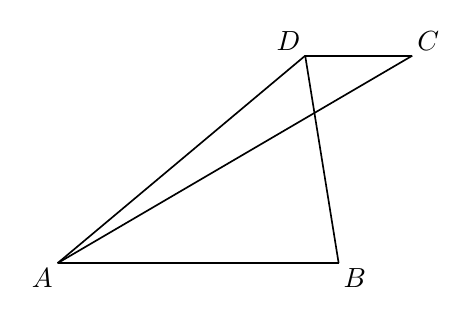
\begin{tikzpicture}[scale=0.85, semithick,
  every node/.style={inner sep=1.5pt}]

  \coordinate (A) at (0.0,0.0);
  \coordinate (B) at (4.2,0.0);
  \coordinate (D) at (3.7,3.1);
  \coordinate (C) at (5.3,3.1);

  \draw (A) -- (B);
  \draw (B) -- (D);
  \draw (D) -- (C);
  \draw (A) -- (D);
  \draw (A) -- (C);

  \node[below left] at (A) {$A$};
  \node[below right] at (B) {$B$};
  \node[above left] at (D) {$D$};
  \node[above right] at (C) {$C$};
\end{tikzpicture}
